\begin{figure}[!htb] 
\centering 
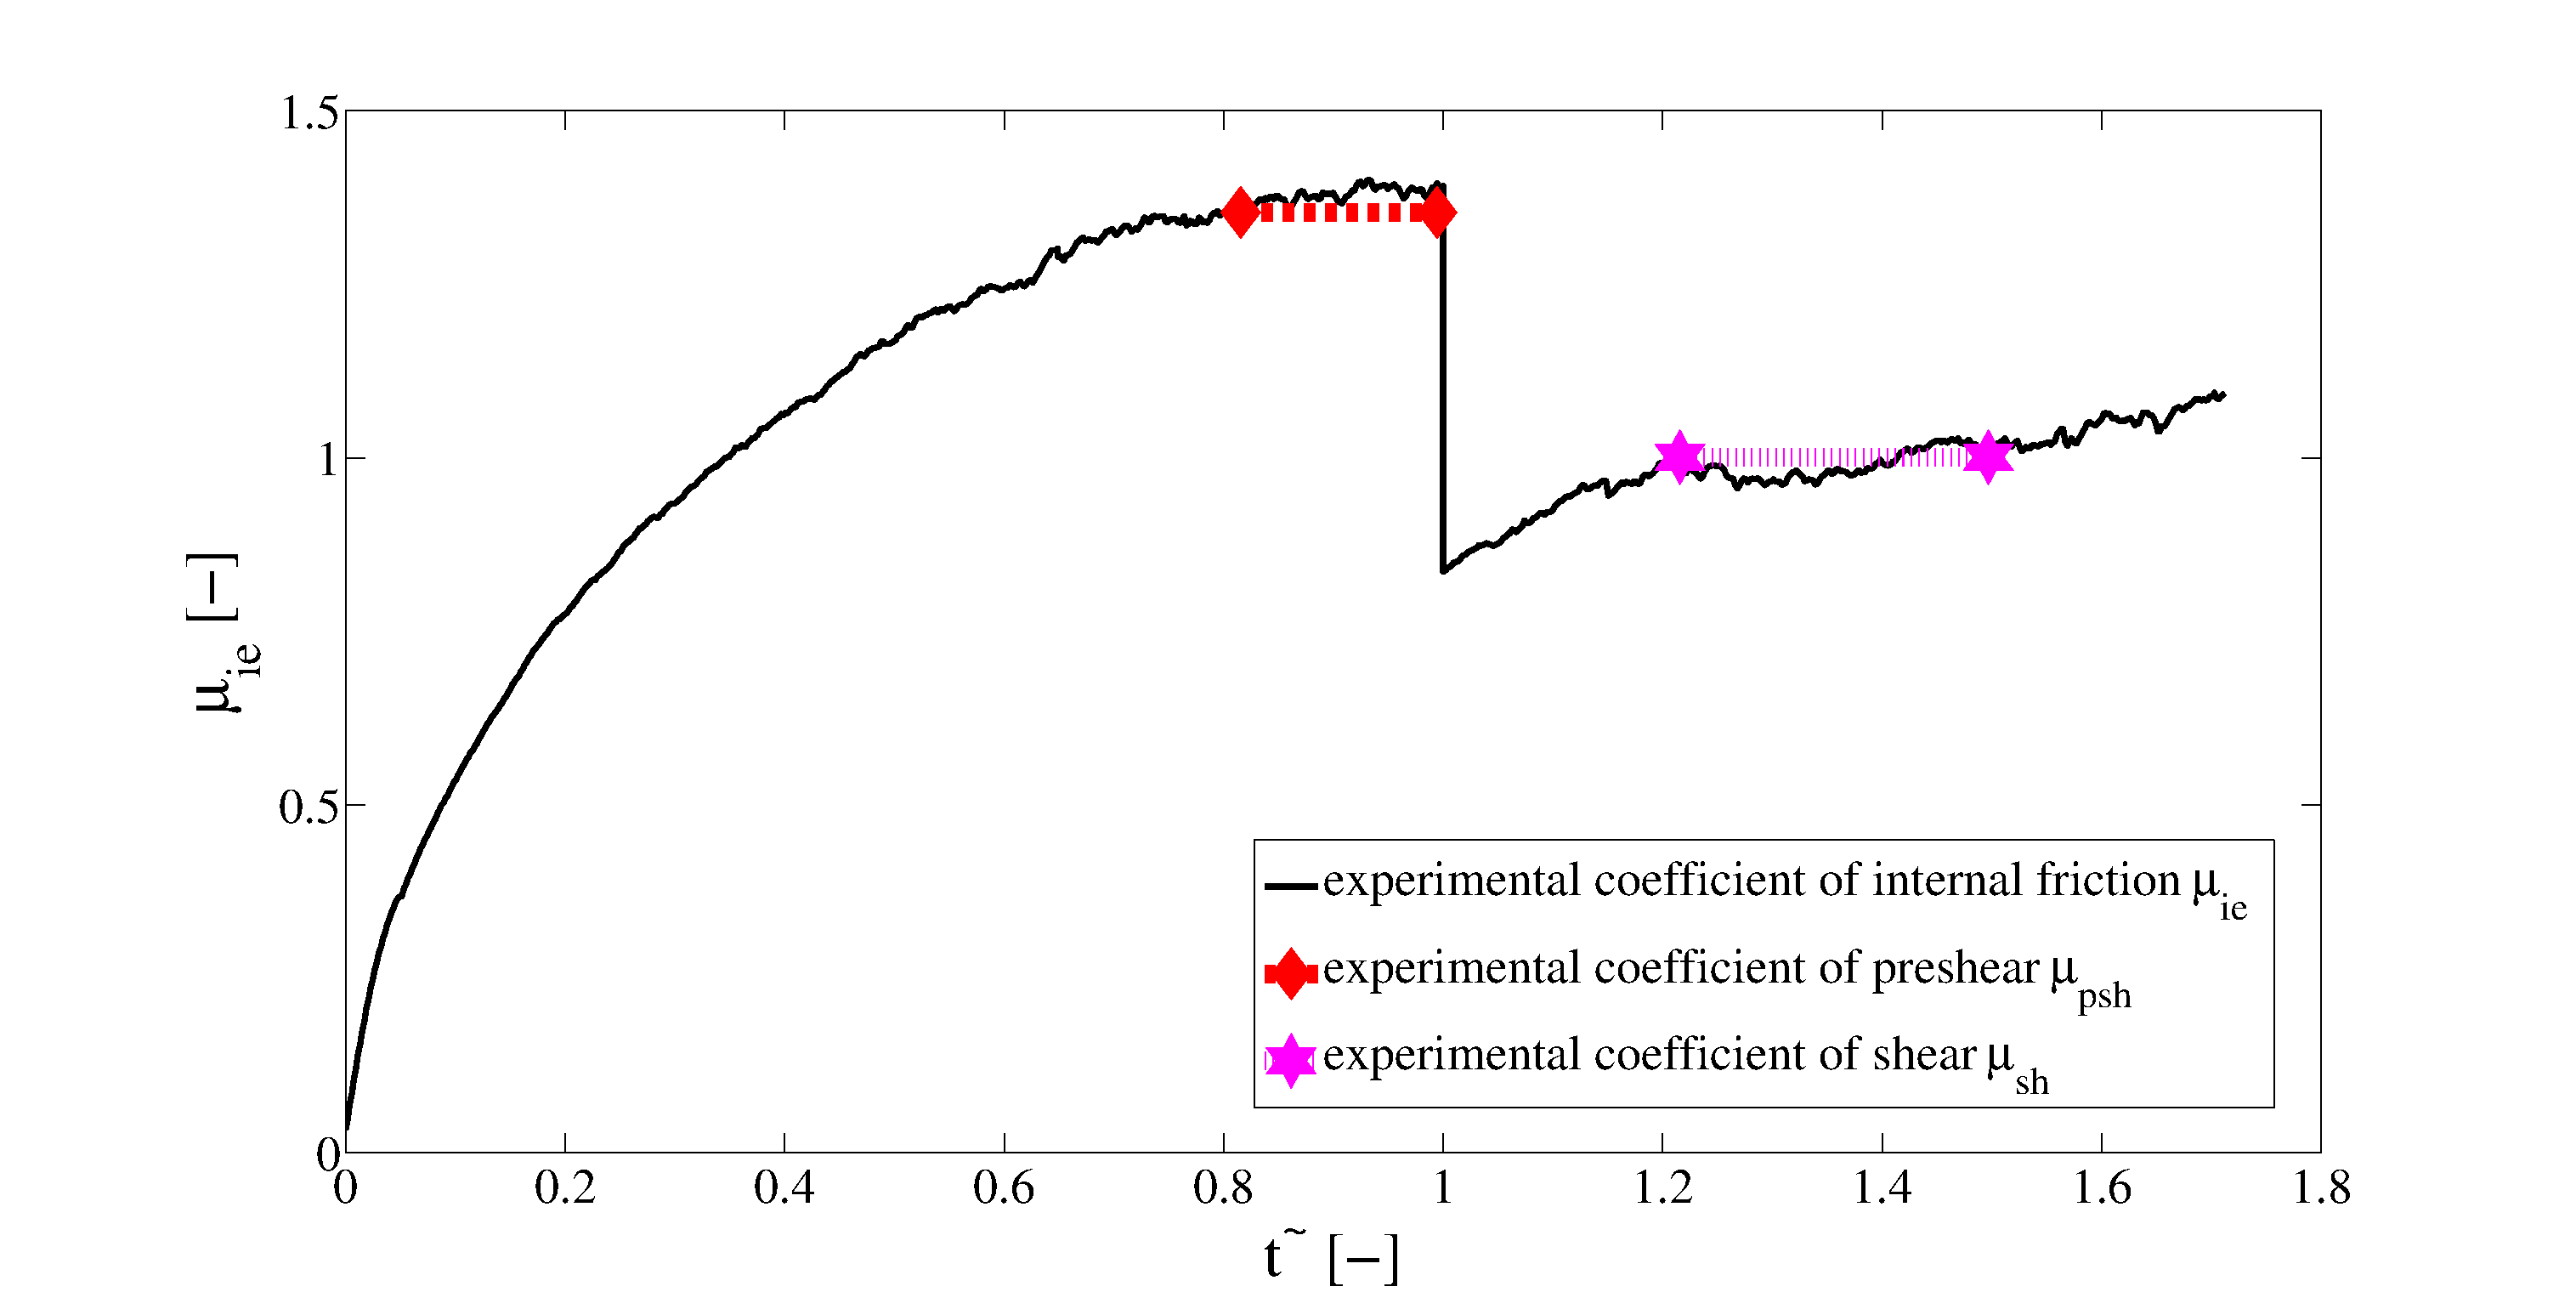
\includegraphics[width=.96\textwidth]{images/original/20experimental} 
\caption[Experimental stress path]{Sample of the experimental stress path for
the Schulze ring shear cell tester.
In the first 300 seconds the $\sigma_n = 2000 ~[Pa]$ is kept constant. After 250
seconds a plateau is reached.
The $\mu_{psh}$ is calculated as average of the $\mu_{ie}$ in this plateau.
Later, the $\sigma_n$ is reduced to $80 \%$ of its initial value.
After approximately 30 seconds, a second plateau starts.
As average of $\mu_{ie}$ in this second plateau we obtain $\mu_{sh}$.
}
\label{fig:20experimental}
\end{figure}

%SCT - experimental - sn = 2000 [Pa]
% \begin{figure}[htp]
%     \centering
%     
\includegraphics[width=.2\textwidth]{images/vitae/lbenvenuti}
%     \caption{OpenMP, MPI, MPI/OpenMP Hybrid runs of Box in a box testcase on 32
%     cores. The OpenMP-only run suffers from limited memory bandwidth in
%     memory-bound algorithms inside of the Modify section of the code. MPI-only has
%     low averaged runtimes for each section, but a very large Other timing, which
%     hints for a large amount of load-imbalance. Hybrid timings are a bit worse
%     on average, but because of better balancing, processes have lower wait times
%     inside of Other timing.}
% 	\label{fig:boxInBoxComparison}
